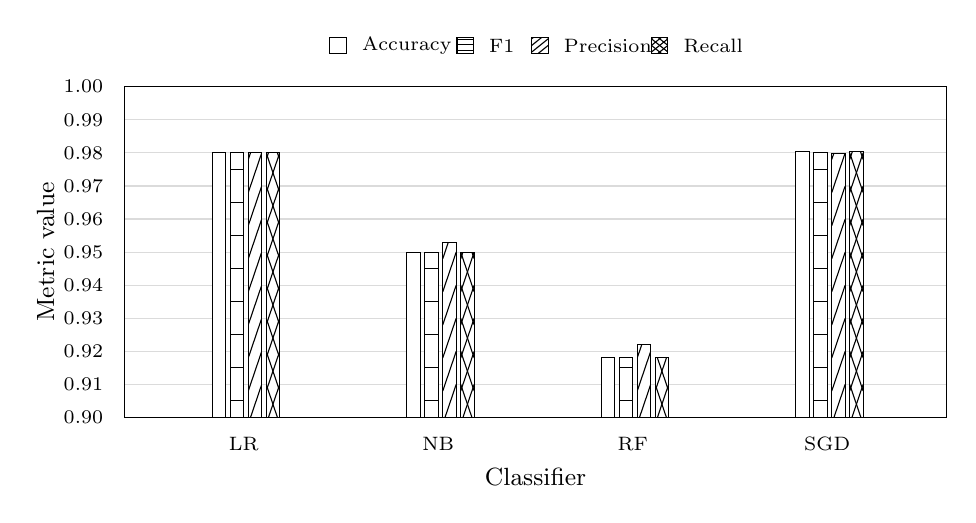
\begin{tikzpicture}[font=\scriptsize,x=0.95cm,y=4.2cm]
  \def\xmin{0}
  \def\xmax{11.0}
  \def\barw{0.18}

  \foreach \yt/\ylab in {
    0.0/0.90,
    0.1/0.91,
    0.2/0.92,
    0.3/0.93,
    0.4/0.94,
    0.5/0.95,
    0.6/0.96,
    0.7/0.97,
    0.8/0.98,
    0.9/0.99,
    1.0/1.00
  }{
    \draw[gray!28] (\xmin,\yt) -- (\xmax,\yt);
    \node[anchor=east] at (-0.15,\yt) {\ylab};
  }
  \draw[black] (\xmin,0) -- (\xmax,0) -- (\xmax,1.0) -- (\xmin,1.0) -- cycle;

  \node[font=\small, rotate=90] at (-1.05,0.5) {Metric value};
  \node[font=\small] at (5.5,-0.18) {Classifier};

  \foreach \x/\name/\acc/\fone/\prec/\rec in {
    1.6/LR/0.800/0.800/0.800/0.800,
    4.2/NB/0.500/0.500/0.530/0.500,
    6.8/RF/0.180/0.180/0.220/0.180,
    9.4/SGD/0.803/0.801/0.798/0.805
  }{
    \node[anchor=north] at (\x, -0.03) {\name};
    \draw[draw=black, fill=white] (\x-0.42,0) rectangle ++(\barw,\acc);
    \draw[draw=black, fill=white] (\x-0.18,0) rectangle ++(\barw,\fone);
    \begin{scope}
      \clip (\x-0.18,0) rectangle ++(\barw,\fone);
      \foreach \yy in {0.05,0.15,0.25,0.35,0.45,0.55,0.65,0.75,0.85}
        \draw[thin] (\x-0.18,\yy) -- ++(\barw,0);
    \end{scope}
    \draw[draw=black, fill=white] (\x+0.06,0) rectangle ++(\barw,\prec);
    \begin{scope}
      \clip (\x+0.06,0) rectangle ++(\barw,\prec);
      \foreach \yy in {-0.12,-0.02,0.08,0.18,0.28,0.38,0.48,0.58,0.68,0.78,0.88}
        \draw[thin] (\x+0.06,\yy) -- ++(\barw,0.12);
    \end{scope}
    \draw[draw=black, fill=white] (\x+0.30,0) rectangle ++(\barw,\rec);
    \begin{scope}
      \clip (\x+0.30,0) rectangle ++(\barw,\rec);
      \foreach \yy in {-0.12,-0.02,0.08,0.18,0.28,0.38,0.48,0.58,0.68,0.78,0.88} {
        \draw[thin] (\x+0.30,\yy) -- ++(\barw,0.12);
        \draw[thin] (\x+0.30,\yy+0.12) -- ++(\barw,-0.12);
      }
    \end{scope}
  }

  \draw[draw=black, fill=white] (2.75,1.10) rectangle ++(0.22,0.05);
  \node[anchor=west] at (3.05,1.125) {Accuracy};
  \draw[draw=black, fill=white] (4.45,1.10) rectangle ++(0.22,0.05);
  \begin{scope}
    \clip (4.45,1.10) rectangle ++(0.22,0.05);
    \foreach \yy in {1.110,1.127,1.144} \draw[thin] (4.45,\yy) -- ++(0.22,0);
  \end{scope}
  \node[anchor=west] at (4.75,1.125) {F1};
  \draw[draw=black, fill=white] (5.45,1.10) rectangle ++(0.22,0.05);
  \begin{scope}
    \clip (5.45,1.10) rectangle ++(0.22,0.05);
    \foreach \yy in {1.085,1.105,1.125,1.145} \draw[thin] (5.45,\yy) -- ++(0.22,0.04);
  \end{scope}
  \node[anchor=west] at (5.75,1.125) {Precision};
  \draw[draw=black, fill=white] (7.05,1.10) rectangle ++(0.22,0.05);
  \begin{scope}
    \clip (7.05,1.10) rectangle ++(0.22,0.05);
    \foreach \yy in {1.085,1.105,1.125,1.145} {
      \draw[thin] (7.05,\yy) -- ++(0.22,0.04);
      \draw[thin] (7.05,\yy+0.04) -- ++(0.22,-0.04);
    }
  \end{scope}
  \node[anchor=west] at (7.35,1.125) {Recall};
\end{tikzpicture}
